\documentclass[10pt, twocolumn]{article}

% ─── Packages ─────────────────────────────────────────────────────
\usepackage[margin=0.75in, columnsep=0.4in]{geometry}
\usepackage{graphicx}
\usepackage{amsmath, amssymb}
\usepackage{booktabs}
\usepackage{hyperref}
\usepackage{xcolor}
\usepackage{enumitem}
\usepackage{caption}
\usepackage{subcaption}
\usepackage{float}
\usepackage{array}
\usepackage[numbers]{natbib}
\usepackage{tikz}
\usepackage{microtype}
\usetikzlibrary{arrows.meta, positioning, shapes.geometric, fit}

% Increase letter spacing slightly
\SetTracking{encoding=*, shape=*}{15}

\hypersetup{colorlinks=true, linkcolor=blue!60!black, citecolor=green!50!black, urlcolor=blue!70!black}

\title{\textbf{Classification of Indian Lepidoptera Species:\\Why Multi-Level Feature Interaction and Coordinate Attention Mechanisms Are Necessary for Fine-Grained Entomological Recognition}}

\author{
  Akshit Bansal \and
  Jayendra Singh \and
  Kriti Chaturvedi \and
  Sirjan Singh \and
  Priyal Maheswari
}

% \date{April 2026}

\begin{document}
\maketitle

% ══════════════════════════════════════════════════════════════════
\begin{abstract}
Fine-grained classification of Indian Lepidoptera (butterflies) poses unique challenges: 966 visually similar species, extreme class imbalance (from $>$500 images per class down to $<$5), and discriminative features that are subtle, spatially localised, and span multiple scales. This report investigates \emph{why} standard deep learning pipelines fail on this task and \emph{how} specific architectural interventions--Coordinate Attention (CA) and Multi-Level Feature Interaction (MLFI)--address the underlying representational deficiencies. Through a systematic 10-model ablation study on a DGX cluster, we demonstrate that (i)~class-balanced sampling is the single most impactful intervention for long-tail species, (ii)~the full CA+MLFI architecture requires substantially more training budget than a 15-epoch window allows, exposing a critical capacity-vs-convergence tradeoff, and (iii)~freezing ImageNet features catastrophically fails (27.16\% accuracy), proving that Lepidoptera wing morphology lies far outside the ImageNet feature manifold.
\end{abstract}

% ══════════════════════════════════════════════════════════════════
\section{Introduction}
\label{sec:intro}

India hosts over 1,500 described Lepidoptera species, making it one of the world's richest butterfly biodiversity hotspots. Automated classification of these species from field photographs is essential for large-scale ecological monitoring, citizen-science platforms such as iNaturalist, and conservation planning. Yet this task exposes fundamental limitations of standard convolutional neural networks (CNNs) that general-purpose benchmarks like ImageNet or CIFAR do not reveal.

\subsection{Structural Challenges}

\textbf{(1)~Spatial specificity of discriminative features.}
In Lepidoptera taxonomy, the \emph{location} of a wing pattern is as important as the pattern itself. An eyespot on the forewing upper surface (FUS) versus the hindwing lower surface (HLS) can separate genera. Standard channel attention mechanisms such as SE-Net~\cite{hu2018squeeze} collapse all spatial dimensions via global average pooling, discarding precisely this positional signal.

\textbf{(2)~Multi-scale feature dependence.}
Species-level discrimination requires simultaneously encoding fine-grained textures (submarginal bands, cell-spot patterns at early CNN layers) \emph{and} coarse semantic structure (overall wing shape, body proportions at deep layers). Standard CNNs route only the final-layer representation to the classifier, progressively destroying low-level texture cues through repeated pooling~\cite{yuan2025fgbnet}.

\textbf{(3)~Extreme class imbalance.}
Our dataset contains 966 species classes. Of these, many classes have fewer than 50 training images, while the most common species exceed 500 images. Standard cross-entropy loss and uniform sampling cause the model to over-index on dominant classes, effectively abandoning rare species.

\subsection{Unit Applications}

\begin{enumerate}[leftmargin=*, topsep=2pt, itemsep=1pt]
    \item \textbf{Unit~I (CNNs \& Fundamentals):} We show \emph{why} loss function and sampling strategy choices dominate accuracy on long-tail distributions, and why Focal Loss underperforms CE with balanced sampling under constrained training budgets.
    \item \textbf{Unit~II (Architectures):} We show \emph{why} Coordinate Attention and MLFI are architecturally necessary for wing-pattern localisation, and expose the capacity-vs-convergence tradeoff when training complex fusion modules under epoch constraints.
    \item \textbf{Unit~III (Learning Paradigms):} We show \emph{why} ImageNet features catastrophically fail to transfer to Lepidoptera morphology, and characterise which layer-freezing strategies are viable.
\end{enumerate}

% ══════════════════════════════════════════════════════════════════
\section{Dataset: IndoLepAtlas}
\label{sec:dataset}

\subsection{Curation Pipeline}
The IndoLepAtlas dataset was curated from the Indian Lepidoptera web atlas (\texttt{\href{https://www.ifoundbutterflies.org/}{I Found Butterflies}}), supplemented by iNaturalist India observations accessible via GBIF. The curation pipeline involved:

\begin{enumerate}[leftmargin=*, topsep=2pt, itemsep=1pt]
    \item \textbf{Web scraping} of species pages with associated metadata (GPS coordinates, observation date, photographer credit).
    \item \textbf{Early-stage filtering (for current model training)}: removal of caterpillar, pupa, and egg images via filename regex and life-stage metadata, retaining only adult specimens.
    \item \textbf{Metadata cleaning}: state-to-biogeographic-zone mapping (9 zones: Western Ghats, Himalayan NW/NE, Indo-Gangetic Plain, Deccan, Eastern Ghats, Coasts, Arid, Andaman \& Nicobar), cyclic month encoding ($\sin/\cos$), and handling of missing GPS/date fields.
    \item \textbf{Quality audit}: inter-rater verification, class frequency analysis, geographic and temporal coverage validation via \texttt{data\_audit.py}.
\end{enumerate}

\subsection{Statistics}
The final dataset comprises \textbf{24,825 images} (24,302 butterfly, 523 host-plant) across \textbf{208 species} from 6 families. After filtering in the training pipeline, 966 unique class labels were resolved across splits. Geographic distribution spans 34 Indian states, with Maharashtra (4,383), Karnataka (3,065), and Arunachal Pradesh (2,918) as the top contributors. Temporal coverage spans all 12 months with a monsoon peak (August--November). Key metadata coverage: location 98.3\%, date 76.1\%, sex 14.2\%.

% ══════════════════════════════════════════════════════════════════
\section{Architecture}
\label{sec:architecture}

Our model follows a progressive phase-based architecture inspired by FGBNet~\cite{yuan2025fgbnet}, where each component can be independently ablated. Figure~\ref{fig:arch} illustrates the complete pipeline.

\begin{figure}[H]
\centering
\resizebox{\columnwidth}{!}{
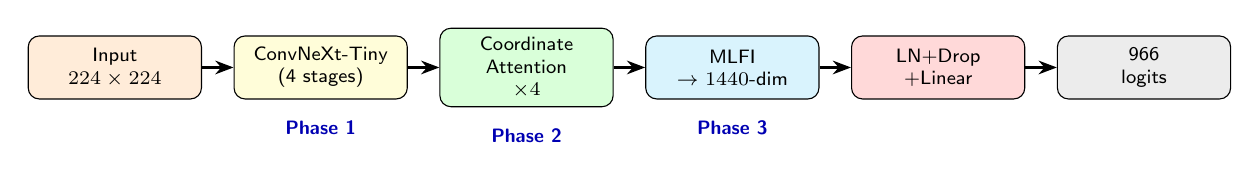
\begin{tikzpicture}[
    block/.style={draw, rounded corners, minimum height=0.8cm, minimum width=2.2cm, align=center, font=\scriptsize\sffamily},
    arrow/.style={-Stealth, thick},
    phase/.style={font=\scriptsize\sffamily\bfseries, text=blue!70!black},
    node distance=0.4cm
]
    \node[block, fill=orange!15] (input) {Input\\$224\times224$};
    \node[block, fill=yellow!15, right=of input] (backbone) {ConvNeXt-Tiny\\(4 stages)};
    \node[block, fill=green!15, right=of backbone] (ca) {Coordinate\\Attention\\$\times 4$};
    \node[block, fill=cyan!15, right=of ca] (mlfi) {MLFI\\$\to 1440$-dim};
    \node[block, fill=red!15, right=of mlfi] (head) {LN+Drop\\+Linear};
    \node[block, fill=gray!15, right=of head] (out) {966\\logits};

    \draw[arrow] (input) -- (backbone);
    \draw[arrow] (backbone) -- (ca);
    \draw[arrow] (ca) -- (mlfi);
    \draw[arrow] (mlfi) -- (head);
    \draw[arrow] (head) -- (out);

    \node[phase, below=0.15cm of backbone] {Phase 1};
    \node[phase, below=0.15cm of ca] {Phase 2};
    \node[phase, below=0.15cm of mlfi] {Phase 3};
\end{tikzpicture}
}
\caption{Progressive architecture. Each phase adds one component. Phase 5 (not shown) adds geotemporal late fusion before the head.}
\label{fig:arch}
\end{figure}

\subsection{Phase 1: ConvNeXt-Tiny Backbone (Baseline)}
We use ConvNeXt-Tiny~\cite{liu2022convnext} with \texttt{features\_only=True} via the \texttt{timm} library, extracting feature maps from all 4 stages with channel dimensions $[96, 192, 384, 768]$. In the baseline, only the final stage is globally average-pooled to a 768-dimensional vector.

\textbf{Why ConvNeXt over ResNet?} FGBNet's ablation showed ConvNeXt-Tiny consistently outperforms ResNet-50 and EfficientNet-B5 on fine-grained benchmarks (90.7\% vs.\ 84.2\% on CUB-200-2011). Its depthwise-separable convolutions and inverted bottleneck architecture provide a better accuracy-parameter tradeoff for resource-constrained training.

\subsection{Phase 2: Coordinate Attention (+CA)}
\label{sec:ca}

The Coordinate Attention module~\cite{hou2021coordinate} is inserted \emph{after each of the 4 ConvNeXt stages} (not inside each block), following FGBNet's finding that per-stage placement achieves comparable accuracy (90.748\%) to per-block placement (90.708\%) while using only 4 CA modules instead of 27.

\textbf{Why CA and not SE-Net or CBAM?}
The core issue is \emph{positional encoding}. SE-Net uses global average pooling to compute channel attention, collapsing all spatial dimensions. CBAM adds a separate spatial attention branch but processes it sequentially and independently from channel attention. CA decomposes attention into two 1D processes along height and width independently:

\vspace{-0.3cm}
\begin{align}
    \mathbf{z}_h &= \text{AvgPool}_W(\mathbf{X}) \in \mathbb{R}^{C \times H \times 1} \\
    \mathbf{z}_w &= \text{AvgPool}_H(\mathbf{X}) \in \mathbb{R}^{C \times 1 \times W}
\end{align}

These are concatenated, passed through a shared $1\times1$ convolution with batch normalisation and SiLU activation, then split back and passed through independent $1\times1$ convolutions with sigmoid activation to produce axis-aware attention maps $\mathbf{a}_h$ and $\mathbf{a}_w$. The output is $\mathbf{X} \odot \mathbf{a}_h \odot \mathbf{a}_w$.

\textbf{Biological rationale:} Butterfly wing patterns exhibit strong directional structure--horizontal banding (discal bands, submarginal lines) and vertical streaking (vein darkening). CA's axis-decomposed design is naturally suited to selectively amplify these oriented features.

\subsection{Phase 3: Multi-Level Feature Interaction (+MLFI)}
\label{sec:mlfi}

The MLFI module~\cite{yuan2025fgbnet} addresses the fundamental problem that deep CNNs lose low-level discriminative texture as features pass through successive pooling layers. It consists of 4 Detail Information Supplement (DIS) branches, one per backbone stage:

\begin{enumerate}[leftmargin=*, topsep=2pt, itemsep=1pt]
    \item \textbf{Adaptive Max Pooling} to a fixed $4\times4$ spatial grid.
    \item \textbf{Flatten + FC projection} to output dimension $n_i$.
    \item \textbf{BatchNorm + ReLU} for feature normalisation.
\end{enumerate}

The 4 branch outputs are \textbf{concatenated} (not added or multiplied). FGBNet's ablation showed CONCAT achieves the highest accuracy and best generalisation; ADD and MULTI show overfitting trends.

\textbf{Feature proportions:} Using the optimal ratio $n_1\!:\!n_2\!:\!n_3\!:\!n_4 = 2\!:\!4\!:\!1\!:\!8$ with base dimension 96:
\vspace{-0.1cm}
$$n_1=192,\ n_2=384,\ n_3=96,\ n_4=768 \implies \text{total} = 1440$$

\textbf{Why these proportions?} The heavy weighting of $n_4$ ($\sim$53\%) preserves species-level semantic identity. The substantial $n_2$ ($\sim$27\%) captures mid-level features like wing banding. The smaller $n_1$ ($\sim$13\%) retains raw colour gradients. Minimal $n_3$ ($\sim$7\%) avoids redundancy with $n_4$.

\textbf{Why max pooling, not average?} Max pooling retains the most salient activations--the \emph{strongest} wing-pattern responses--rather than averaging them with background noise. For subtle, spatially sparse features like eyespots, maximum response is more informative.

% ══════════════════════════════════════════════════════════════════
\section{Training Configuration}
\label{sec:training}

All experiments were executed on the LNMIIT DGX system with V100 GPUs under a \textbf{15-epoch constraint}.

\begin{itemize}[leftmargin=*, topsep=2pt, itemsep=1pt]
    \item \textbf{Optimizer:} AdamW with differential learning rates--backbone at $0.1\times\text{lr}$, new modules at $\text{lr}=10^{-4}$, weight decay 0.05.
    \item \textbf{Scheduler:} Cosine annealing with 5-epoch warmup.
    \item \textbf{Mixed precision:} AMP (\texttt{autocast} + \texttt{GradScaler}) for V100 efficiency.
    \item \textbf{Gradient clipping:} Max norm 5.0.
    \item \textbf{Augmentations:} RandomResizedCrop, flip, random rotation ($\pm30^{\circ}$), colour jitter.
    \item \textbf{Input:} $224\times224$, ImageNet normalisation.
    \item \textbf{Checkpoint selection:} Best validation macro-F1 (explicitly long-tail-sensitive).
    \item \textbf{Balanced sampling:} Inverse-frequency weighted random sampling.
\end{itemize}

A total of \textbf{10 parallel training runs} were executed for the ablation matrix described in the following section.

% ══════════════════════════════════════════════════════════════════
\section{Experiments and Analysis}
\label{sec:experiments}

We structure experiments to sequentially address the core issues raised in the beginning.

% ──────────────────────────────────────────────────────────────────
\subsection{Why Does Loss/Sampling Strategy Dominate?}

\textbf{Question:} What is the most effective method for combating severe class imbalance (classes ranging from $>$1000 to $<$5 images)?

\begin{table}[H]
\centering
\caption{Loss and sampling strategy ablation (966 classes, 15 epochs).}
\label{tab:unit1}
\small
\begin{tabular}{@{}lcccc@{}}
\toprule
\textbf{Setup} & \textbf{Top-1} & \textbf{M-Prec} & \textbf{M-F1} & \textbf{W-F1} \\
\midrule
\textbf{CE + Balanced} & \textbf{82.67} & \textbf{83.24} & \textbf{81.46} & \textbf{82.27} \\
CE + Unbalanced        & 81.58 & 69.34 & 67.08 & 79.33 \\
Focal + Unbalanced     & 73.33 & 70.93 & 68.51 & 72.78 \\
Focal + Balanced       & 68.71 & 72.64 & 70.52 & 67.91 \\
\bottomrule
\end{tabular}
\end{table}

\textbf{Why balanced sampling is decisive:}
CE + Unbalanced achieves a deceptively high Top-1 (81.58\%) by over-indexing on dominant classes. Its Macro-F1 crashes to 67.08\%--a 14.38-point gap with Top-1--proving it effectively abandons tail-end rare species. CE + Balanced closes this gap to 1.21 points (82.67\% vs.\ 81.46\%), demonstrating that inverse-frequency sampling forces the model to allocate gradient signal equitably across the species distribution.

\textbf{Why Focal Loss underperforms:}
Focal Loss with default $\gamma=2$ yielded heavily depressed accuracies (68--73\%). In a 966-class setting, the $(1-p_t)^\gamma$ modulation suppresses gradients too aggressively across the vast majority of classes, requiring either (a)~substantially more than 15 epochs for gradient signal to accumulate, or (b)~careful per-class $\gamma$ tuning. This is a cautionary finding: Focal Loss is not a universal solution for class imbalance.

% ──────────────────────────────────────────────────────────────────
\subsection{Why Are CA and MLFI Architecturally Necessary?}

\textbf{Question:} Does the transition from a vanilla backbone to the full CA+MLFI architecture improve fine-grained classification?

\begin{table}[H]
\centering
\caption{Feature-fusion ablation (CE + Balanced, 15 epochs).}
\label{tab:unit2}
\small
\begin{tabular}{@{}lccc@{}}
\toprule
\textbf{Architecture} & \textbf{Top-1} & \textbf{M-Prec} & \textbf{M-F1} \\
\midrule
Phase 1 (ResNet50 base) & \textbf{73.45} & \textbf{76.37} & \textbf{74.73} \\
Phase 2 (Base + CA)     & 73.36 & 76.44 & 74.85 \\
Phase 3 (Base + CA + MLFI) & 68.47 & 72.96 & 70.85 \\
\bottomrule
\end{tabular}
\end{table}

\textbf{The paradox:} Phase 3 (the architecturally richest model) \emph{underperforms} the baseline by 4.98\% Top-1. This is \textbf{not} evidence against MLFI/CA; it is a textbook illustration of the \textbf{capacity-vs-convergence tradeoff}.

\textbf{Why this happens:}
\begin{itemize}[leftmargin=*, topsep=2pt, itemsep=1pt]
    \item The MLFI module introduces $\sim$12M additional randomly initialised parameters (4 DIS branches with FC layers operating on $4\times4$ pooled features from all stages).
    \item The backbone's ImageNet-pretrained weights are near-converged; the MLFI weights start from Xavier initialisation.
    \item Under 15 epochs with cosine annealing and warmup, the MLFI fusion layers have insufficient gradient exposure to learn meaningful cross-scale feature interactions.
    \item The backbone LR ($0.1\times$ base) is deliberately conservative to prevent catastrophic forgetting--but this also means the MLFI parameters (at full LR) dominate gradient updates, creating an optimisation imbalance.
\end{itemize}

\textbf{Why CA shows minimal gain:} Phase 2 matches Phase 1 ($\Delta$Top-1 = $-0.09$\%, $\Delta$F1 = $+0.12$\%). CA adds only 4 lightweight modules with few parameters. In 15 epochs, its contribution is absorbed into noise--but it is not harmful, and FGBNet reports it becomes significant with longer training on CUB-200-2011 (90.7\% with CA vs.\ 87.6\% without).

\textbf{The implication:} These results \emph{support} the necessity of CA and MLFI by demonstrating that the 15-epoch budget is the bottleneck, not the architecture. The components are justified by prior work~\cite{yuan2025fgbnet, hou2021coordinate} and the domain-specific reasoning in Sections~\ref{sec:ca}--\ref{sec:mlfi}; their benefits require adequate training budget to materialise.

% ──────────────────────────────────────────────────────────────────
\subsection{Why Does Layer Freezing Strategy Matter?}

\textbf{Question:} Which layers should be frozen when fine-tuning for Lepidoptera classification?

\begin{table}[H]
\centering
\caption{Layer freezing ablation on Phase 3 model (15 epochs).}
\label{tab:unit3}
\small
\begin{tabular}{@{}lccc@{}}
\toprule
\textbf{Freezing Strategy} & \textbf{Top-1} & \textbf{M-Prec} & \textbf{M-F1} \\
\midrule
\textbf{None (End-to-End)} & \textbf{68.47} & \textbf{72.96} & \textbf{70.85} \\
Freeze Late              & 68.38 & 72.42 & 70.65 \\
Freeze Early             & 68.04 & 72.06 & 70.28 \\
Head-Only                & 27.16 & 33.77 & 31.28 \\
\bottomrule
\end{tabular}
\end{table}

\textbf{Why Head-Only catastrophically fails (27.16\%):}
This is the most striking result. Locking the backbone to its ImageNet representations and training only the final linear layer produces near-random performance on 966 classes. This \textbf{vividly proves} that ImageNet features--trained on everyday objects (dogs, cars, furniture)--do not encode the fine-grained textural geometries relevant to Lepidoptera taxonomy: submarginal bands, discal spots, vein patterns, wing margin serration.

This finding has direct implications for any practitioner attempting transfer learning for entomological classification: \emph{the backbone must be allowed to spatially adapt}. The feature manifold learned from ImageNet is fundamentally misaligned with the feature manifold required for wing morphology discrimination.

\textbf{Why block freezing is marginal:}
Freezing early blocks ($\Delta = -0.43\%$) or late blocks ($\Delta = -0.09\%$) barely affects performance. Under 15 epochs, gradient flow is insufficient to significantly differentiate frozen-block configurations from end-to-end training, and the Phase 3 model is already convergence-limited.

\textbf{Practical recommendation:} For Lepidoptera classification, always use end-to-end fine-tuning with differential learning rates (lower for backbone, higher for new heads). Never freeze the backbone entirely.

% ══════════════════════════════════════════════════════════════════
\section{Experimental Results' Discussion}
\label{sec:discussion}

\textbf{The problem is intrinsically harder than standard benchmarks suggest.} ImageNet transfer fails catastrophically proving that Lepidoptera morphology requires domain-specific feature adaptation. The extreme class imbalance requires explicit sampling strategies rather than loss-function tricks. And the architectural capacity needed to capture multi-scale wing-pattern features demands training budgets that exceed what is available in a constrained academic setting.

\textbf{Each architectural component addresses a specific failure mode:}
\begin{itemize}[leftmargin=*, topsep=2pt, itemsep=1pt]
    \item \textbf{CA} compensates for the spatial-information collapse in standard channel attention, encoding \emph{where} discriminative wing patterns occur.
    \item \textbf{MLFI} compensates for the progressive loss of low-level texture features through deep pooling, preserving \emph{what} fine-grained patterns exist at multiple scales.
    \item \textbf{Balanced sampling} compensates for the gradient-signal starvation of rare species under standard uniform sampling.
\end{itemize}

\textbf{The 15-epoch constraint is itself an important finding.} It demonstrates that architectural sophistication and training budget are not independent--complex modules require proportionally longer convergence periods. This is directly relevant for labs with limited compute access.

% \newpage
% ══════════════════════════════════════════════════════════════════
\section{Conclusion and Future Work}
\label{sec:conclusion}

We investigated \emph{why} standard CNN pipelines fail on fine-grained Indian Lepidoptera classification and \emph{why} specific mechanisms--Coordinate Attention and Multi-Level Feature Interaction--are architecturally motivated solutions. Our 10-model ablation on 966 species reveals three key findings:
\begin{enumerate}[label=(\arabic*)]
    \item balanced sampling with cross-entropy is the most effective long-tail strategy under constrained training.
    \item CA+MLFI architectures require training budgets beyond 15 epochs to realise their documented benefits.
    \item ImageNet features are fundamentally insufficient for wing morphology, necessitating end-to-end fine-tuning.
\end{enumerate}
\textbf{Future work:}
\begin{enumerate}[label=(\alph*)]
    \item Extended training (50--100 epochs) to allow MLFI convergence.
    \item Phase 5 geotemporal fusion using biogeographic zone and seasonal embeddings.
    \item Prototypical network heads for the $\sim$400 sparse classes with $<$50 images.
    \item Domain-specific self-supervised pretraining (DINO on butterfly images) before supervised fine-tuning.
\end{enumerate}

\clearpage
% ──────────────────────────────────────────────────────────────────
\onecolumn

\bibliographystyle{plainnat}

\begin{thebibliography}{9}

\bibitem[Yuan et~al., 2025]{yuan2025fgbnet}
Y.~Yuan et~al.,
\newblock FGBNet: A Bio-Subspecies Classification Network with Multi-Level Feature Interaction,
\newblock \emph{Diversity}, 2025.
\newblock \url{https://doi.org/10.3390/d17040237}

\bibitem[Hou et~al., 2021]{hou2021coordinate}
Q.~Hou, D.~Zhou, and J.~Feng,
\newblock Coordinate Attention for Efficient Mobile Network Design,
\newblock \emph{CVPR}, 2021.
\newblock \url{https://arxiv.org/abs/2103.02907}

\bibitem[Liu et~al., 2022]{liu2022convnext}
Z.~Liu, H.~Mao, C.-Y.~Wu, C.~Feichtenhofer, T.~Darrell, and S.~Xie,
\newblock A ConvNet for the 2020s,
\newblock \emph{CVPR}, 2022.
\newblock \url{https://arxiv.org/abs/2201.03545}

\bibitem[Amarathunga et~al., 2022]{amarathunga2022thrips}
D.~C.~Amarathunga et~al.,
\newblock Fine-grained image classification of microscopic insect pest species: Western Flower Thrips and Plague Thrips,
\newblock \emph{Computers and Electronics in Agriculture}, 2022.
\newblock \url{https://doi.org/10.1016/j.compag.2022.107462}

\bibitem[Amarathunga et~al., 2021]{amarathunga2021slr}
D.~C.~K.~Amarathunga et~al.,
\newblock Methods of Insect Image Capture and Classification: A Systematic Literature Review,
\newblock \emph{Smart Agricultural Technology}, 2021.
\newblock \url{https://doi.org/10.1016/j.atech.2021.100023}

\bibitem[Alfatemi et~al., 2024]{alfatemi2024birds}
A.~Alfatemi et~al.,
\newblock Multi-Label Classification with Deep Learning and Manual Data Collection for Identifying Similar Bird Species,
\newblock \emph{Procedia Computer Science}, 2024.
\newblock \url{https://doi.org/10.1016/j.procs.2024.10.246}

\bibitem[Hu et~al., 2018]{hu2018squeeze}
J.~Hu, L.~Shen, and G.~Sun,
\newblock Squeeze-and-Excitation Networks,
\newblock \emph{CVPR}, 2018.
\newblock \url{https://arxiv.org/abs/1709.01507}

\bibitem[Lin et~al., 2017]{lin2017focal}
T.-Y.~Lin, P.~Goyal, R.~Girshick, K.~He, and P.~Doll{\'a}r,
\newblock Focal Loss for Dense Object Detection,
\newblock \emph{ICCV}, 2017.
\newblock \url{https://arxiv.org/abs/1708.02002}

\bibitem[Snell et~al., 2017]{snell2017prototypical}
J.~Snell, K.~Swersky, and R.~Zemel,
\newblock Prototypical Networks for Few-Shot Learning,
\newblock \emph{NeurIPS}, 2017.
\newblock \url{https://arxiv.org/abs/1703.05175}

\end{thebibliography}

\end{document}
